\documentclass[a4 paper]{article}
% Set target color model to RGB



\usepackage[inner=2.0cm,outer=2.0cm,top=2.5cm,bottom=2.5cm]{geometry}
\usepackage{setspace}
\usepackage[rgb]{xcolor}
\usepackage{verbatim}
\usepackage{subcaption}
\usepackage{amsgen,amsmath,amstext,amsbsy,amsopn,tikz,amssymb,tkz-linknodes}
\usepackage{fancyhdr}
\usepackage[colorlinks=true, urlcolor=blue,  linkcolor=blue, citecolor=blue]{hyperref}
\usepackage[colorinlistoftodos]{todonotes}
\usepackage{rotating}
%\usetikzlibrary{through,backgrounds}

\usepackage{lmodern}
\usepackage[T1]{fontenc}
\usepackage[capposition=top]{floatrow}
\usepackage{hyperref}
\usepackage{graphicx}
\graphicspath{ {images/} }
\usepackage{booktabs}
\usepackage{changepage}
\usepackage{float}
\usepackage{fancyvrb}







\hypersetup{%
pdfauthor={Nick Korbit},%
pdftitle={Homework},%
%pdfkeywords={Tikz,latex,bootstrap,uncertaintes},%
pdfcreator={PDFLaTeX},%
pdfproducer={PDFLaTeX},%
}
%\usetikzlibrary{shadows}
% \usepackage[francais]{babel}
\usepackage{booktabs}


\newcommand{\ra}[1]{\renewcommand{\arraystretch}{#1}}

\newtheorem{thm}{Theorem}[section]
\newtheorem{prop}[thm]{Proposition}
\newtheorem{lem}[thm]{Lemma}
\newtheorem{cor}[thm]{Corollary}
\newtheorem{defn}[thm]{Definition}
\newtheorem{rem}[thm]{Remark}
\numberwithin{equation}{section}

\newcommand{\homework}[6]{
   \pagestyle{myheadings}
   \thispagestyle{plain}
   \newpage
   \setcounter{page}{1}
   \noindent
   \begin{center}
   \framebox{
      \vbox{\vspace{2mm}
    \hbox to 6.28in { {\bf ISYE 6420:~Bayesian Statistics \hfill {\small #2}} }
       \vspace{6mm}
       \hbox to 6.28in { {\Large \hfill #1  \hfill} }
       \vspace{6mm}
       \hbox to 6.28in { {\it Instructor: {\rm #3} \hfill Name: {\rm #5}, gtID: {\rm #6}} }
       %\hbox to 6.28in { {\it TA: #4  \hfill #6}}
      \vspace{2mm}}
   }
   \end{center}
   \markboth{#5 -- #1}{#5 -- #1}
   \vspace*{4mm}
}

\newcommand{\problem}[2]{~\\\fbox{\textbf{Problem #1}}\newline\newline}
\newcommand{\subproblem}[1]{~\newline\textbf{(#1)}}
\newcommand{\D}{\mathcal{D}}
\newcommand{\Hy}{\mathcal{H}}
\newcommand{\VS}{\textrm{VS}}
\newcommand{\solution}{~\newline\textbf{\textit{(Solution)}} }

\newcommand{\bbF}{\mathbb{F}}
\newcommand{\bbX}{\mathbb{X}}
\newcommand{\bI}{\mathbf{I}}
\newcommand{\bX}{\mathbf{X}}
\newcommand{\bY}{\mathbf{Y}}
\newcommand{\bepsilon}{\boldsymbol{\epsilon}}
\newcommand{\balpha}{\boldsymbol{\alpha}}
\newcommand{\bbeta}{\boldsymbol{\beta}}
\newcommand{\0}{\mathbf{0}}



%%%%%%%%%%%%%%%%%%%%%%%%%%%%%%%%%%%%%%%%
%%			 Document				  %%
%%%%%%%%%%%%%%%%%%%%%%%%%%%%%%%%%%%%%%%%


\begin{document}
	
\homework{Homework \#6}{Spring 2020}{Roshan Vengazhiyil, Brani Vidakovic}{}{Nick Korbit}{903263968}


%%%%%%%%%%%%%%%%%%%%%%%%%%%%%%%%%%%%%%%%
%%			 Problem 1				  %%
%%%%%%%%%%%%%%%%%%%%%%%%%%%%%%%%%%%%%%%%

\problem{1}

\textbf{a)} Let $x_1$ be the time after injection
and $y$ be the temperature. We model $y$ as
a normally distributed variable with 
mean $\mu$ and precision $\tau$:

$$
y \sim \mathcal{N}\left(\mu,\tau\right)
$$

We then model $\mu$ as a linear regression:

$$
\hat{\mu}=\alpha+\beta x_{1}
$$

We also set non-informative for 
$\alpha$, $\beta$ and $tau$:

\begin{align*}
\alpha&\sim\mathcal{N}\left(0,0.001\right)\\\beta&\sim\mathcal{N}\left(0,0.001\right)\\\tau&\sim\mathcal{G}a\left(0.001,0.001\right)
\end{align*}


Given observed 10 data points we 
specify an OpenBUGS model as

\begin{Verbatim}
# Training
for (i in 1:n) {
mu[i] <- alpha + beta*time[i]
temp[i] ~ dnorm(mu[i], tau)	
}

# Priors
tau ~ dgamma(0.001, 0.001)
alpha ~ dnorm(0, 0.001)
beta ~ dnorm(0, 0.001)
\end{Verbatim} 

In the observed data points we have one 
missing value for $x_1$. Assuming that 
missingness happened at random and 
noticing that $x_1$ are arranged 
in the ascending order, we can 
put a uniform distribution $\mathcal{U}(56,70)$
on the missing 5th value:

\begin{Verbatim}
time[5] ~ dunif(56, 70)
\end{Verbatim} 


Then we specify calculation for $R^2$.
Since we have 2 independent variables, 
we adjust $SSE$ by $(n-2)$:

\begin{Verbatim}
# R^2
sigma2 <- 1/tau
sse <- (n-2)*sigma2
for(i in 1:n){
ctemp[i] <- temp[i] - mean(temp[])
}
sst <- inprod(ctemp[], ctemp[]) 
BR2 <- 1 - sse/sst
BR2adj <- 1 - (n-1) * sigma2 / sst
\end{Verbatim} 



We initialize values for the priors as:
\begin{Verbatim}
list(alpha = 0, beta = 0, tau=1) 
\end{Verbatim} 



Let's now run an OpenBUGS simulation. We burn
the first 10000 observation and update the model 
with the next 100000 samples. First, we 
investigate stats:

\begin{figure}[H]
	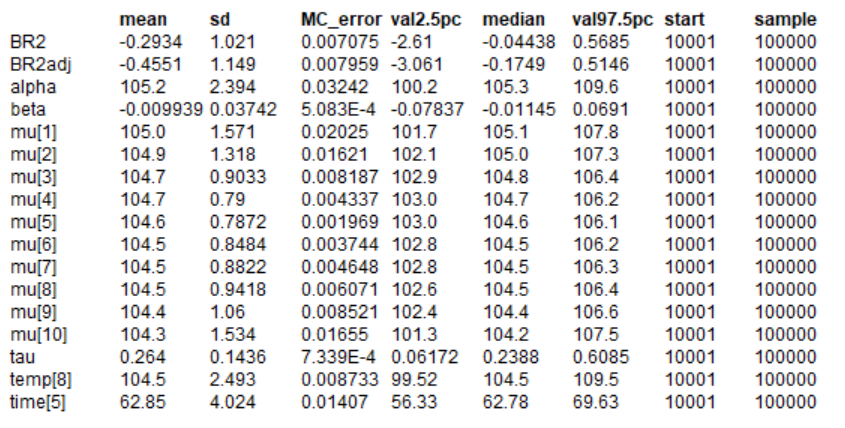
\includegraphics[scale=1.0]{q1}
	\centering
	%	\caption{cdf .}
	\label{q1}
\end{figure}


We notice that both $R^2$ and $R^2_{adj}$
have negative values, meaning that in principle
we are better off with just setting an average 
of $y_i$ as our prediction. We have also 
automatically inferred values for the 
missing data -- $x_5$ and $y_8$, 
with $y_8$ averaging at $104.5$: 

\begin{figure}[H]
	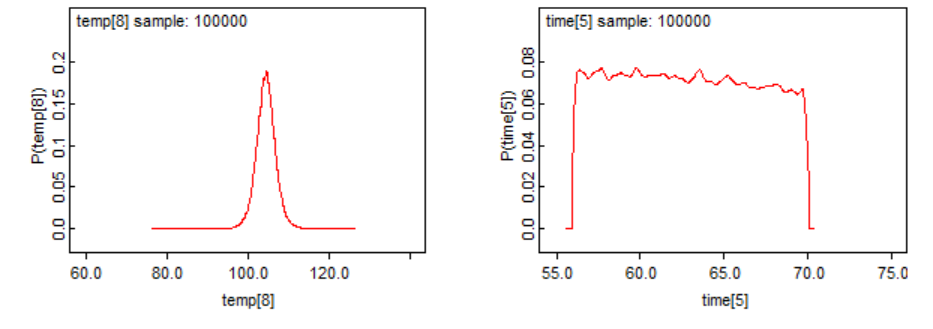
\includegraphics[scale=1.0]{q1_2}
	\centering
	%	\caption{cdf .}
	\label{q1_2}
\end{figure}


The 95\% credible set for the slope 
$\beta$ is around $(-0.08, 0.07)$, so that
 $0$ is inside the set. \\



\textbf{b)} We now expand our model 
with a new vaiable -- 
time after injection squared. So that:

$$
\hat{\mu}=\alpha+\beta_1 x_{1} +\beta_2 x_{1}^2
$$

Or in OpenBUGS terms:

\begin{Verbatim}
# Training
for (i in 1:n) {
mu[i] <- alpha + beta1*time[i] + beta2*time2[i]
temp[i] ~ dnorm(mu[i], tau)	
}

# Priors
tau ~ dgamma(0.001, 0.001)
alpha ~ dnorm(0, 0.001)
beta1 ~ dnorm(0, 0.001)
beta2 ~ dnorm(0, 0.001)
\end{Verbatim}


We also model missing values
as uniform distributions:

\begin{Verbatim}
time[5] ~ dunif(56, 70)
time2[5] ~ dunif(3136, 4900)
\end{Verbatim} 



Since we have 3 independent variables, 
we adjust $SSE$ by $(n-3)$.
Let's now run an OpenBUGS simulation. We burn
the first 10000 observation and update the model 
with the next 100000 samples. First, we 
investigate stats:

\begin{figure}[H]
	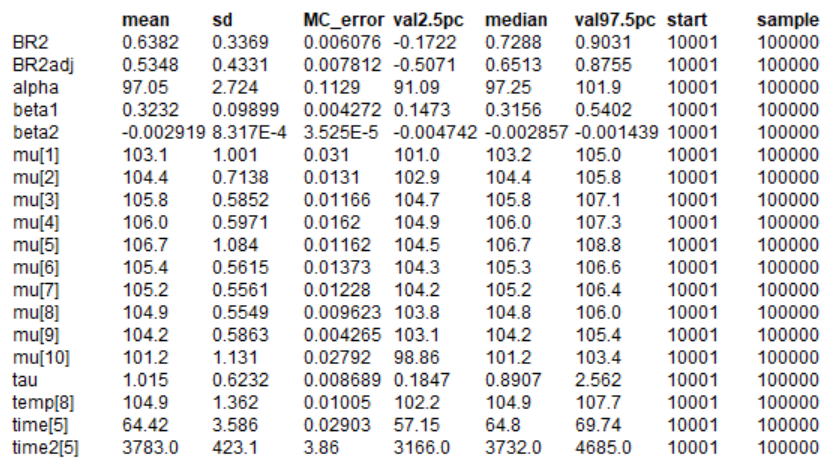
\includegraphics[scale=1.0]{q1_3}
	\centering
	%	\caption{cdf .}
	\label{q1_3}
\end{figure}


We notice that means for both $R^2$ and $R^2_{adj}$
are much higher now, $0.64$ and $0.53$ respectively.
So including a time squared feature is a good 
idea and that alone significantly boosts model
performance.

We have also 
automatically inferred values for the 
missing data -- $x_5$, $x_5^2$ and $y_8$, 
with $y_8$ averaging at $104.9$: 

\begin{figure}[H]
	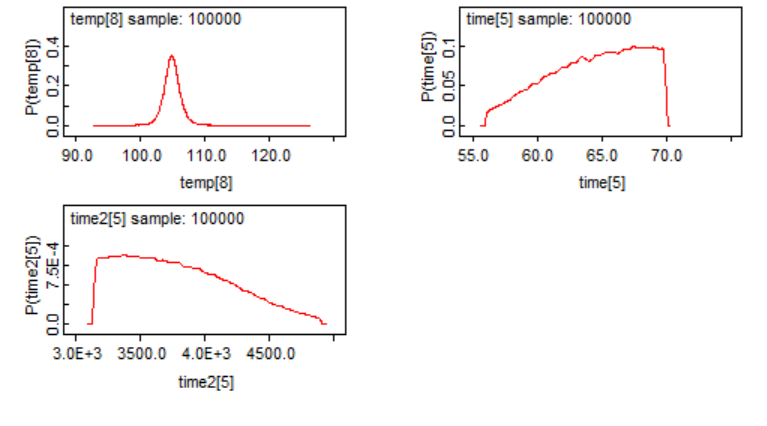
\includegraphics[scale=1.0]{q1_4}
	\centering
	%	\caption{cdf .}
	\label{q1_4}
\end{figure}


The 95\% credible set for the slope 
$\beta_1$ is around $(0.15, 0.54)$ and
$(-0.005, -0.001)$ for beta $\beta_2$. 
So that 
$0$ is not inside the sets. \\



\textbf{Note}: the full OpenBUGS code is available 
at \textit{rabbits1.odc} and \textit{rabbits2.odc}
in the attached archive. \\ \\

 




%%%%%%%%%%%%%%%%%%%%%%%%%%%%%%%%%%%%%%%%
%%			 Problem 2				  %%
%%%%%%%%%%%%%%%%%%%%%%%%%%%%%%%%%%%%%%%%

\problem{2}

Assuming observed times are exponentially distributed 
with non-informative priors,
let's first define the OpenBUGS model:

\begin{Verbatim}
for(i in 1:n) {                          
time[i] ~ dexp(lambda[i])I(time.cen[i],)
lambda[i] <- exp(beta0 + beta1*group[i])
}	

beta0 ~ dnorm(0.0, 0.0001)
beta1 ~ dnorm(0.0, 0.0001)
\end{Verbatim} 

We also can derive the estimators
for the expected time until recurrence (the 
bigger value, the better treatment is). 
$\mu_0$ is the mean time for placebo (no treatment)
and $\mu_1$ is the mean time for chemotherapy:

\begin{Verbatim}
mu0 <- exp(-beta0)
mu1 <- exp(-beta0-beta1)
diff <- mu1-mu0
ph1 <- step(diff)
\end{Verbatim} 

Let's now run an OpenBUGS simulation. We start 
with burning 
the first 10000 observation and update the model 
with the next 100000 samples. First, 
we investigate the stats:

\begin{figure}[H]
	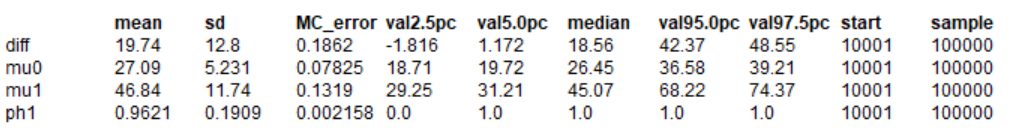
\includegraphics[scale=1.0]{q2}
	\centering
	%	\caption{cdf .}
	\label{q2}
\end{figure}



\begin{figure}[H]
	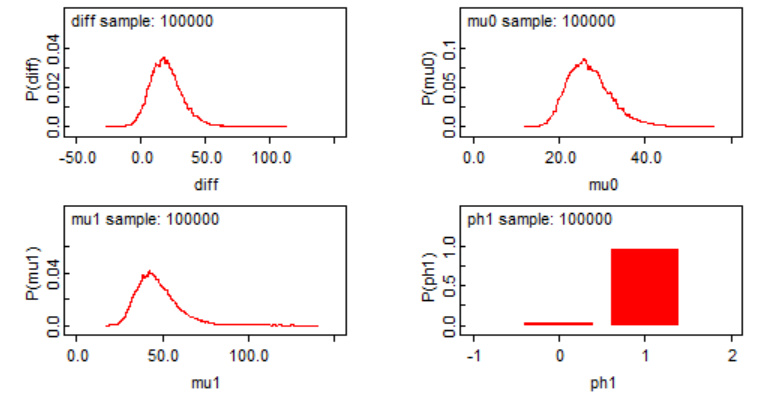
\includegraphics[scale=1.0]{q2_2}
	\centering
	\label{q2_2}
\end{figure}




We notice that the expected time until 
cancer recurrence is far more 
larger in case of the chemotherapy --
$46.8$ months vs $27.1$ months (placebo 
treatment). Constructing 
a 90\% credible set for the difference
in means $\mu_1-\mu_0$
will yield us $(1.17, 36.6)$. 

Next, we test the hypothesis 
$H_1: \mu_1-\mu_0$. The OpenBUGS 
simulation estimates the probability 
of $H_1$ as 96.2\%, so that we 
accept $H_1$ hypothesis. 




Since 90\% credible set for the difference
in means is always positive 
and the probability 
of $H_1: \mu_1-\mu_0$ hypothesis is 96.2\%, we can conclude 
that chemotherapy is beneficial for the 
patient. The treatment extends the time
to recurrence by 19 months on average.  \\











\textbf{Note}: the full OpenBUGS code is available 
at \textit{bladderc0.odc} in the attached archive.



%%%%%%%%%%%%%%%%%%%%%%%%%%%%%%%%%%%%%%%%
%%			 Bibliography			  %%
%%%%%%%%%%%%%%%%%%%%%%%%%%%%%%%%%%%%%%%%

\begin{thebibliography}{9}


\bibitem{stat}\label{stat} 
Engineering Biostatistics: An Introduction using MATLAB and WinBUGS. 
Brani Vidakovic - Wiley Series in Probability and Statistics.

\end{thebibliography}



\end{document} 